\section*{Task 1 -- Forecasting across heterogeneous sensors}

\paragraph{Run.} Every number and figure below comes from one fresh top-to-bottom execution of
\path{task1/Assignment1.ipynb} with \texttt{PA1\_PRESET=full}, data seed 0 and model seed 0, on an RTX~4070 Laptop GPU. The run took 280\,s, and every notebook check passed. ``Established'' means stations 1--3 and ``held-out'' means station~4. Each claim below names its population and its split (training, validation or test).

\paragraph{Implementations.}
\begin{itemize}
  \item \textbf{\texttt{RawAttentionForecaster.forward}} embeds the context ($[B,1,L]\!\to\![B,d,L]$), transposes back and adds the learned position table. It then applies both encoder blocks and the final LayerNorm, flattens $[B,L,d]$, and maps it to $[B,H]$ with the forecast head.
  \item \textbf{\texttt{SeriesDecomposition.forward}} replicates the first and last values $\lfloor m/2\rfloor$ times along time, averages with a stride-1 \texttt{avg\_pool1d} over time for every channel, and returns $(x-T,\,T)$.
  \item \textbf{\texttt{aggregate\_delays}} builds, per example, the source index $(t-\tau_j)\bmod L$, gathers the $K$ shifted copies of the values with \texttt{torch.gather}, and sums them weighted by $\alpha_j$. It is fully vectorized and differentiable in both values and weights.
\end{itemize}

% ---------------------------------------------------------------------------------------------
\subsection*{Response 1A -- predicted, measured and revised ordering}

\textbf{Prediction} (recorded in \path{task1/predictions_before_running.md} before any cell ran; drafted with AI assistance, see the appendix):
established, period-routed ridge $<$ Raw Attention $<$ shared ridge $\approx$ sensor-specific ridge;
held-out, period-routed ridge $<$ Raw Attention $<$ shared ridge (sensor-specific ridge unavailable).

\begin{table}[H]\centering\small
\caption{Output 1.1, validation. RMSE in \ms, MSE in \mss. Columns A, B and C give RMSE by product.}
\resizebox{\linewidth}{!}{\begin{tabular}{lrrrrrrrrrrr}
\toprule
 & \multicolumn{5}{c}{Established stations 1--3} & \multicolumn{5}{c}{Held-out station 4} & \\
\cmidrule(lr){2-6}\cmidrule(lr){7-11}
Model & RMSE & MSE & A & B & C & RMSE & MSE & A & B & C & Params \\
\midrule
Shared ridge          & 0.767 & 0.588 & 0.805 & 0.854 & 0.621 & 0.876 & 0.767 & 0.909 & 0.982 & 0.713 & 4{,}608 \\
Sensor-specific ridge & 0.768 & 0.590 & 0.804 & 0.852 & 0.630 & --    & --    & --    & --    & --    & 13{,}824 \\
Period-routed ridge   & \textbf{0.166} & \textbf{0.028} & 0.181 & 0.164 & 0.152 & \textbf{0.173} & \textbf{0.030} & 0.184 & 0.182 & 0.150 & 59{,}904 \\
Raw Attention         & 0.408 & 0.166 & 0.376 & 0.434 & 0.410 & 0.577 & 0.333 & 0.565 & 0.548 & 0.616 & 368{,}368 \\
\bottomrule
\end{tabular}}
\end{table}

\textbf{Measured} (validation). The ordering holds in both populations and for every product.
\begin{itemize}
  \item \textbf{Period routing is far ahead of everything else.} On established stations its RMSE is 4.6$\times$ lower than shared ridge (0.166 vs 0.767) and 2.5$\times$ lower than Raw Attention (0.408). Raw Attention halves shared ridge's error ($-$47\%).
  \item \textbf{Station identity buys nothing.} On established stations, sensor-specific ridge equals shared ridge (0.768 vs 0.767) with three times the parameters.
  \item \textbf{Moving to station~4 costs very different amounts.} From established to held-out RMSE, period-routed ridge loses 4\% (0.166$\to$0.173), shared ridge 14\% (0.767$\to$0.876) and Raw Attention 41\% (0.408$\to$0.577).
  \item \textbf{Product effects.} Routed ridge is nearly flat across products in both populations (0.150--0.184). The unconditioned ridges are worst on Product~B and best on Product~C in both populations. Raw Attention has no consistent product ranking: established stations are worst on B (0.434), station~4 worst on C (0.616).
\end{itemize}

\textbf{Revision.} The ordering stands. I underestimated two magnitudes: routing's margin over Raw Attention, and Raw Attention's 41\% loss on station~4. I had also expected no station-4 loss for the linear shared map.

\textbf{Explanation by assumptions.}
\begin{itemize}
  \item \textbf{Shared ridge} applies one operator to every pace from 14 to 36 samples, so least squares settles on a compromise.
  \item \textbf{Sensor-specific ridge} conditions on a variable that does not determine the pace, since every station runs every pace. It therefore makes the same compromise.
  \item \textbf{Period-routed ridge} conditions on the variable that actually changes. Within a 1.5-sample band a linear map is nearly ideal for a sinusoid plus a smooth ramp. It does not use station identity, so it transfers almost unchanged to station~4.
  \item \textbf{Raw Attention} can build a context-dependent rule, but it must learn it from about 1{,}950 drift-dominated training windows. Its features are tied to the training stations' amplitudes and offsets, which is consistent with its large validation loss on station~4.
  \item \textbf{Shared ridge's 14\% station-4 loss is proportionate.} Its compromise error is a fixed fraction of the vibration it mis-predicts. Station~4 vibrates at 2.15\ms, against a mean of 1.88\ms\ for stations 1--3, a ratio of 1.14, which matches its validation error ratio $0.876/0.767 = 1.14$.
\end{itemize}

% ---------------------------------------------------------------------------------------------
\subsection*{Response 1B -- why the rule must depend on the context}

\begin{figure}[H]\centering
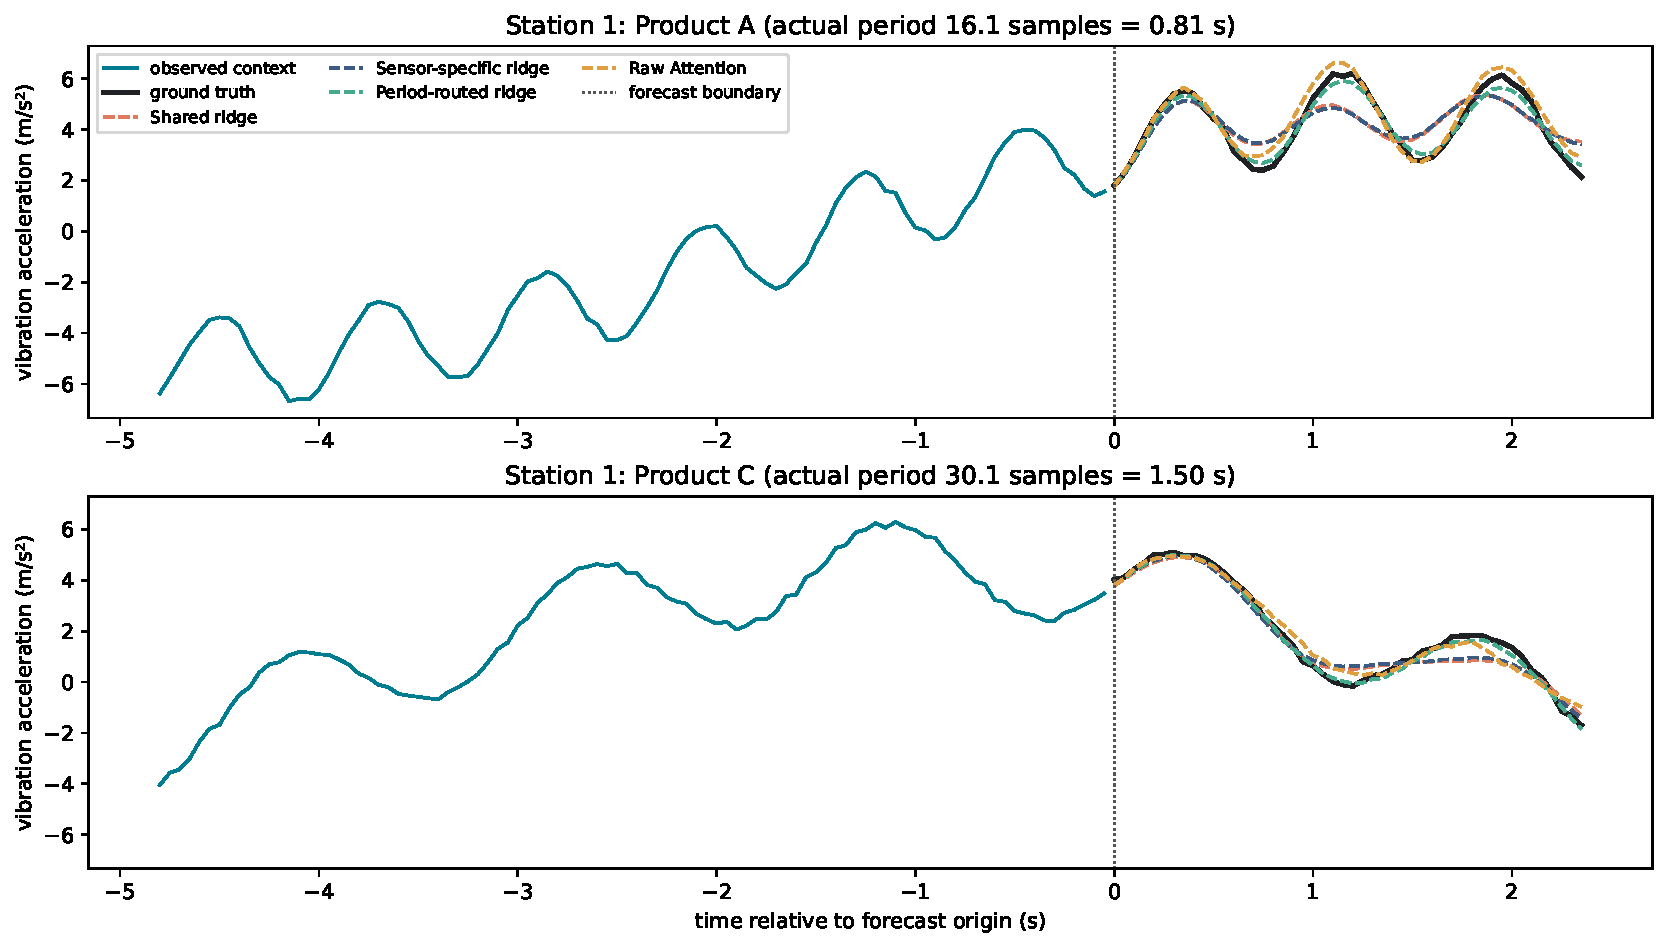
\includegraphics[width=0.83\linewidth]{figures/task1/1.2-1.pdf}
\caption{Output 1.2: station 1 (established) in a Product A validation run ($P=16.1$) and a Product C validation run ($P=30.1$).}
\end{figure}

\textbf{The compromise in the forecast} (station 1, validation). In the Product A window, shared and sensor-specific ridge get the first half-cycle's phase roughly right, but the oscillation then \emph{shrinks}. Predicted peaks reach about 4.9\ms\ against a true 6.2\ms, and predicted troughs sit near 3.5\ms\ against a true 2.4\ms. Their window RMSE is 0.78, against 0.23 for routed ridge. In the Product C window, the second, slower bump is flattened into a plateau (window RMSE 0.45 against 0.15).

A single $\hat W$ in equation (8) has no variable that selects the phase advance per step, so least squares averages the continuations of incompatible paces. Under squared error, the best response to phase uncertainty is the conditional mean, and an average of out-of-phase sinusoids has a smaller amplitude. That is the damping we see.

\begin{figure}[H]\centering
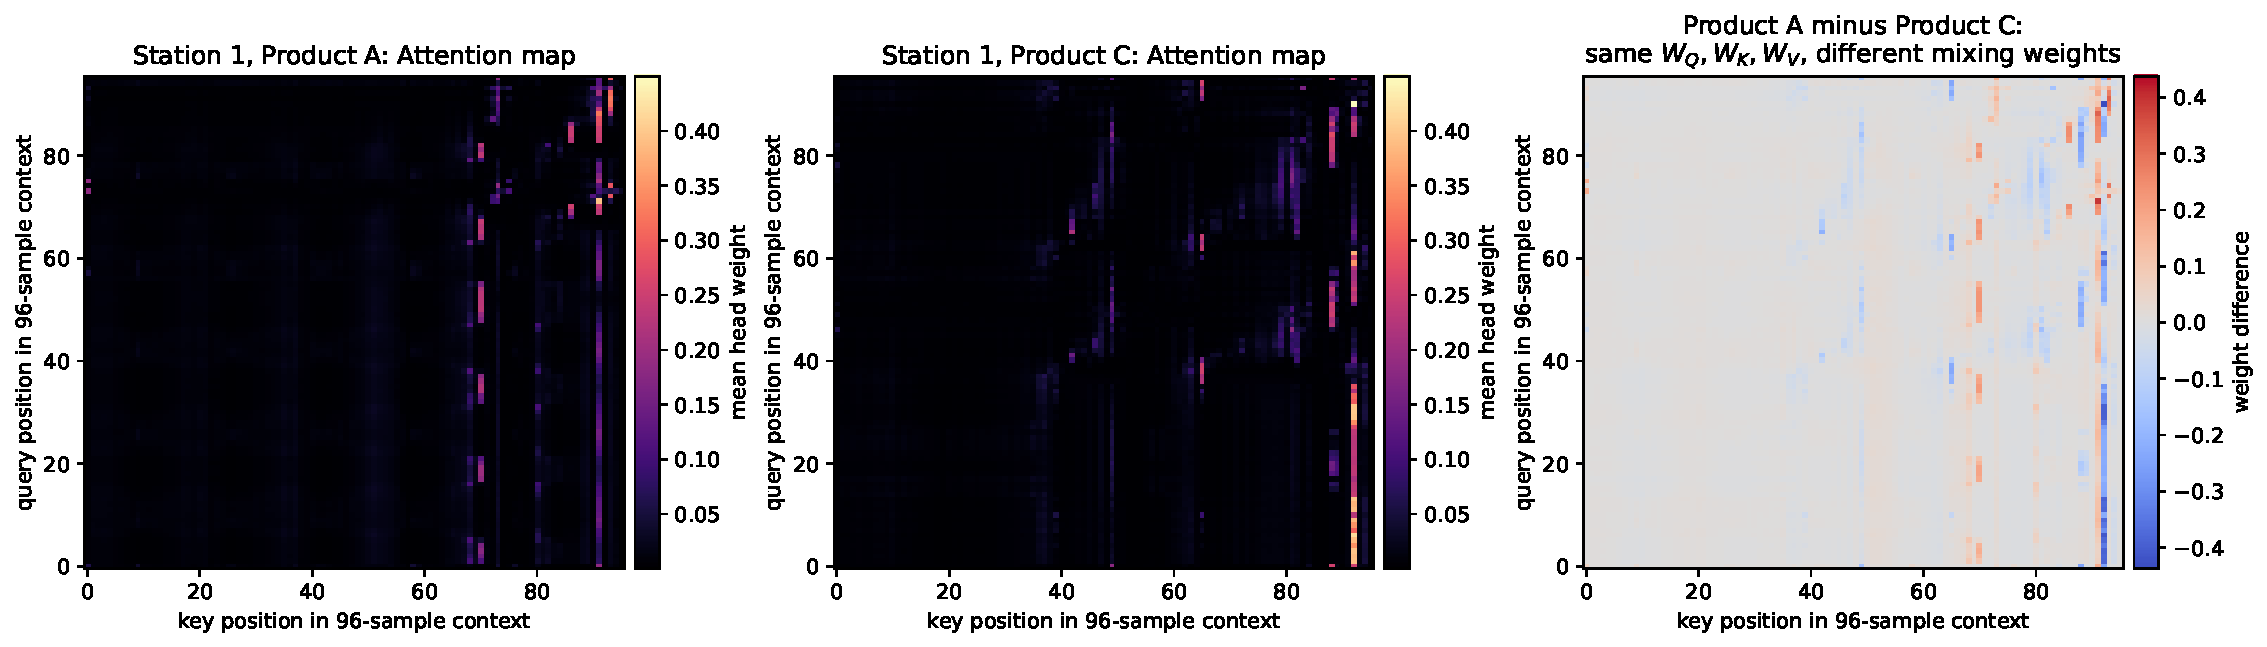
\includegraphics[width=\linewidth]{figures/task1/1.3-1.pdf}
\caption{Output 1.3: first-layer Attention (mean over heads) for the same two validation windows of station 1, and their difference.}
\end{figure}

\textbf{How the same projections produce different mixing} (station 1, validation). $W_Q, W_K, W_V$ are fixed after training, but the $96\times96$ weights $\operatorname{softmax}(QK^\top/\sqrt{d_h})$ are recomputed from each window. Both maps put their weight on the most recent 30 or so keys, but on different columns: Product~A favours keys near 70 and 90--94, while Product~C spreads weight across keys near 42, 49, 65 and 80--93. The difference map has mean $|\Delta| = 0.013$ but a maximum of 0.44, so some queries move 44\% of their weight to different positions. Because the output is $A(X)V$, each window gets its own value-mixing operator, without refitting and without a router. Ridge applies the same $\hat W$ to both windows. This figure shows only that the mixing depends on the input; it is not evidence that Attention recovered the physical period.

% ---------------------------------------------------------------------------------------------
\subsection*{Response 2 -- separating slow structure from repetition}

\begin{figure}[H]\centering
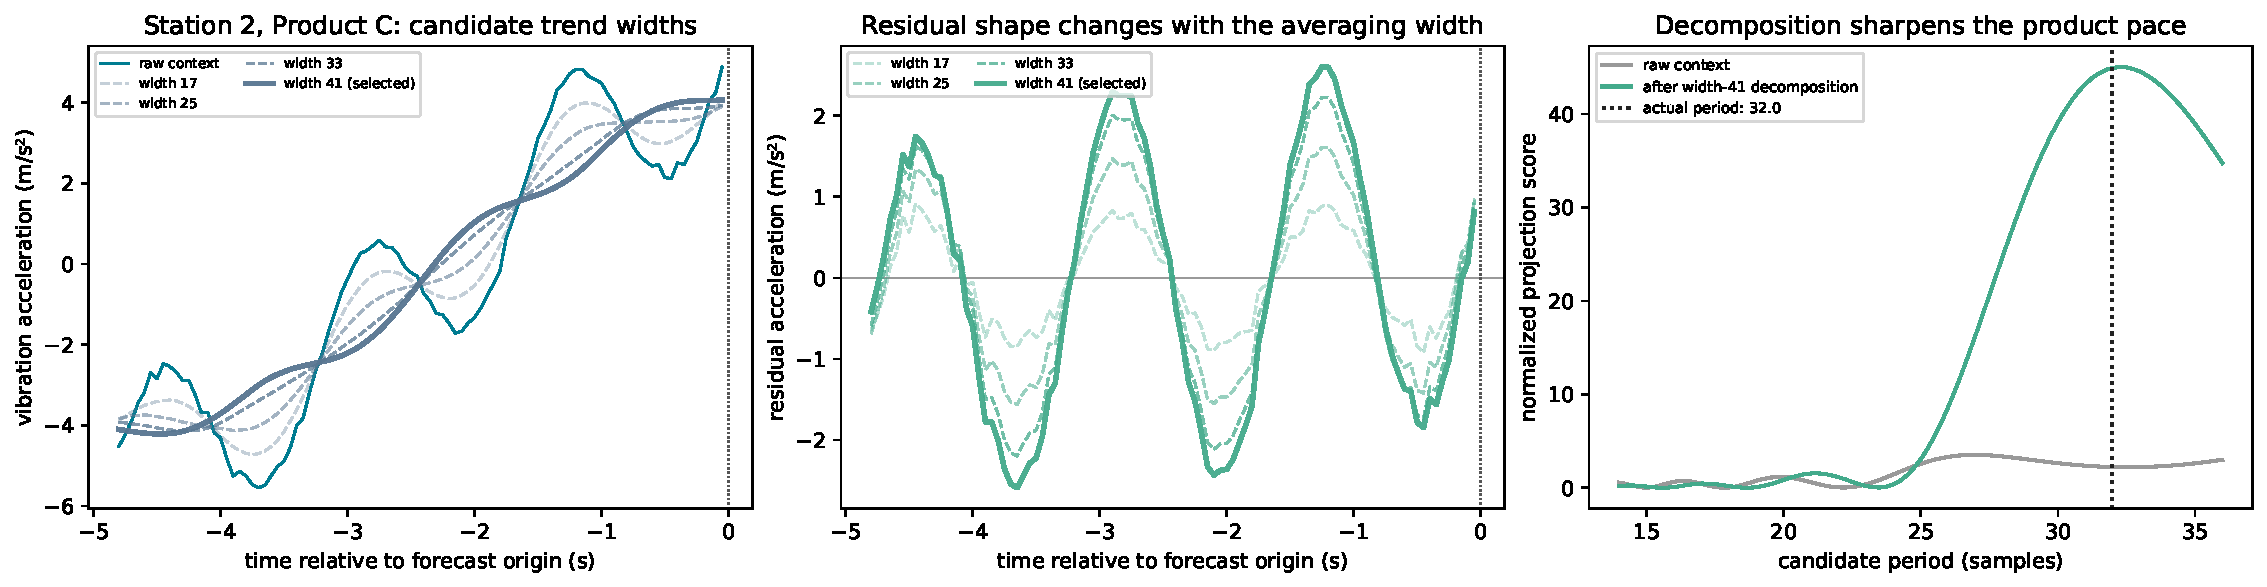
\includegraphics[width=\linewidth]{figures/task1/2.1-1.pdf}\\[2pt]
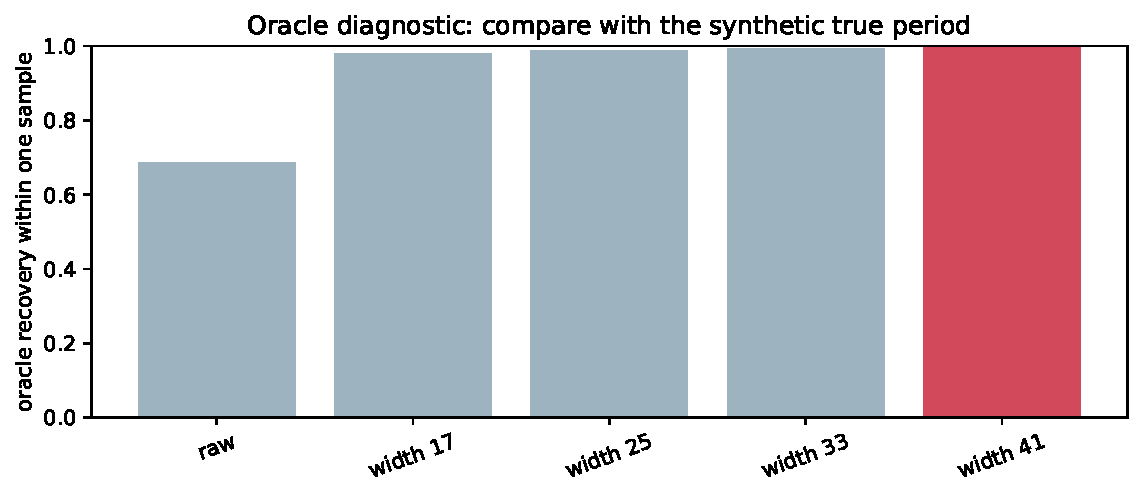
\includegraphics[width=0.55\linewidth]{figures/task1/2.2-1.pdf}
\caption{Output 2.1 (top): candidate widths on the validation window where the raw period estimate is most wrong (station 2, Product C, $P=32$). Output 2.2 (bottom): oracle period recovery on training windows of the established stations.}
\end{figure}

\textbf{Selected width and what changes.} The selected width is $m=41$.
\begin{itemize}
  \item \textbf{Output 2.1} (station 2, validation window). Narrow widths let the trend follow the vibration. At $m=17$ the trend wiggles with the 32-sample cycle, and the remainder keeps only a residual standard deviation of 0.58\ms. At $m=41$ the trend is a smooth ramp and the remainder carries the full oscillation (standard deviation 1.57\ms). The raw window's projection score has no clear peak; after the width-41 split it peaks sharply at the true period of 32.
  \item \textbf{Output 2.2} (established stations, training windows). Period recovery within one sample rises from 68.7\% on raw windows to 98.0\%, 98.9\%, 99.3\% and 99.85\% for widths 17, 25, 33 and 41.
  \item \textbf{Output 2.3} (validation). Decomposition lowers Raw Attention's RMSE from 0.408 to 0.299 on established stations ($-$27\%) and from 0.577 to 0.439 on station~4 ($-$24\%). The error falls for every product in both populations: on established stations A 0.376$\to$0.276, B 0.434$\to$0.329 and C 0.410$\to$0.289; on station~4 A 0.565$\to$0.381, B 0.548$\to$0.471 and C 0.616$\to$0.459.
  \item \textbf{Contrasting cases} (station 4, validation). In the largest-gain window, the raw model's forecast lags in phase and the decomposed model corrects it. In the smallest-gain window, decomposition slightly hurts: the forecast drifts out of phase late in the horizon.
\end{itemize}

\begin{figure}[H]\centering
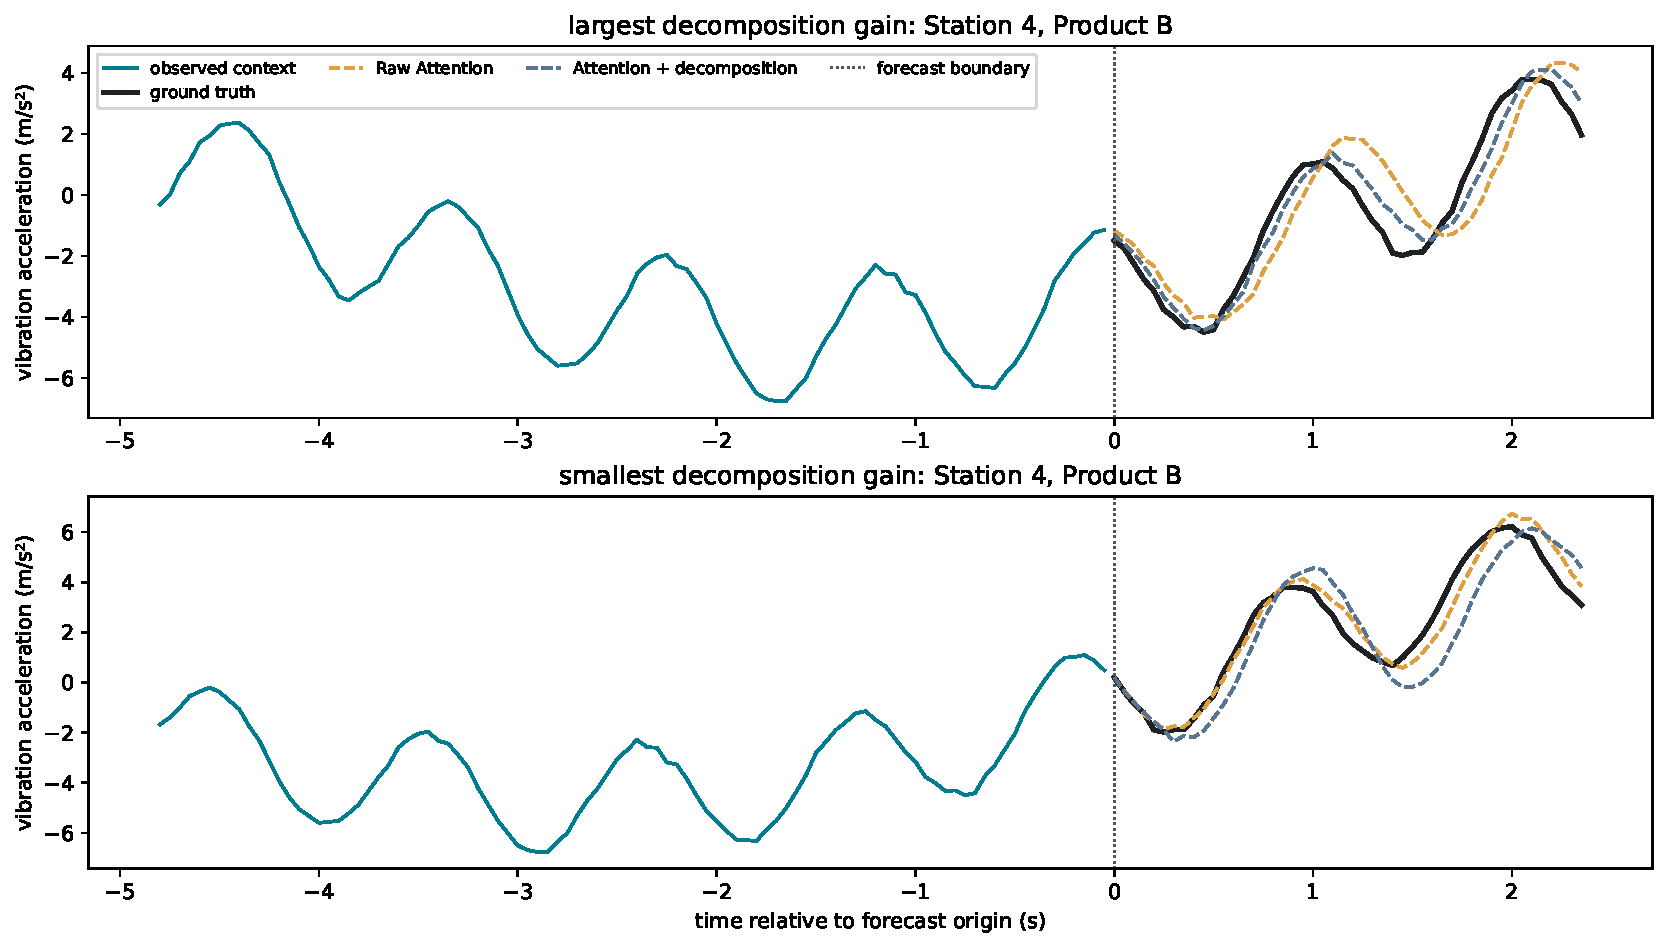
\includegraphics[width=0.8\linewidth]{figures/task1/2.3-1.pdf}
\caption{Output 2.3: validation windows with the largest and smallest decomposition gain (both on held-out station 4).}
\end{figure}

\textbf{Why a moving average suits this world.} The data are a 240-sample drift plus one 14--36-sample vibration, a wide separation of time scales. A centered average of width $m$ scales a sinusoid of period $P$ by $H(P)=\sin(\pi m/P)/(m\sin(\pi/P))$. For $m=41$ that means $H\approx0.95$ at $P=240$, while the vibration bands are attenuated to about 10--18\% on average. The drift therefore goes almost entirely to the linear trend head, and the mixer sees an almost pure oscillation. The filter has no parameters, is linear and differentiable, and introduces no phase shift.

\textbf{Why the oracle diagnostic is a good selector here.} In this simulator the true period of every window is known, so we can measure directly whether a width exposes the repetition, which is the property the mixers depend on. The measurement uses training windows from established stations only, never touches validation or test, and never feeds the true period to a model. It is also cheap, needing no training per width. A deployed system would have no true period and would need a proxy such as validation error.

\textbf{Where the bias fails.} It fails on an abrupt level shift, such as a load step. A width-41 average smears a step of height $h$ into a 41-sample ramp and leaves a $\pm h/2$ artifact in the remainder. It also fails at the context edges when the drift curves: replicate padding assumes the signal is flat beyond the edge, so at the last sample the trend lags a ramp of slope $a$ by $a\,q(q+1)/(2m)\approx5.1a$. An alternative is STL (loess-based decomposition; Cleveland et al., 1990), which fits a smooth trend robustly and handles curvature better. It encodes a known seasonal period and gives up the parameter-free, period-agnostic behaviour.

% ---------------------------------------------------------------------------------------------
\subsection*{Response 3 -- mixing by temporal delay}

\textbf{Output 3.1} confirms that the supplied FFT scores equal a direct circular correlation on $[1,3,1,3]$: $(4,-4,4,-4)$.

\textbf{Aggregation check.} My \texttt{aggregate\_delays} reproduces the notebook's worked example exactly: $z=[35,15,25,25]$ for $v=[10,20,30,40]$, delays $[1,3]$ and weights $[\tfrac34,\tfrac14]$. Since $z_0=\tfrac34 v_3+\tfrac14 v_1=35$ (not 25), position $t$ reads from $t-\tau$ as equation (6) requires. The notebook's gradient and wrap-around checks also pass.

\begin{figure}[H]\centering
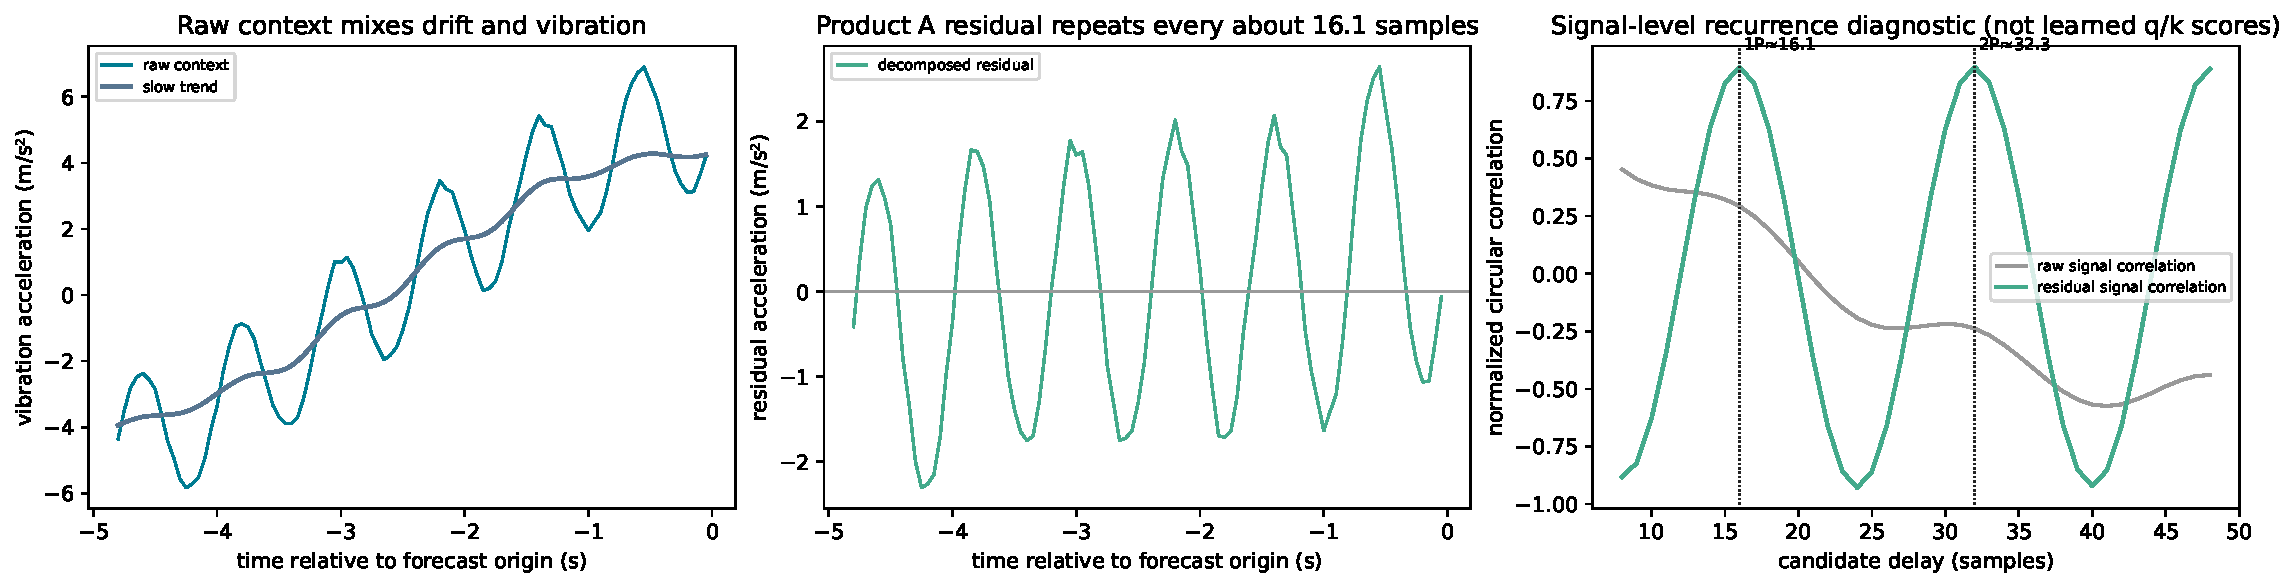
\includegraphics[width=\linewidth]{figures/task1/3.2-1.pdf}
\caption{Output 3.2: signal-level recurrence diagnostic for one validation window (station 2, Product A, $P=16.13$). These are not the model's learned q/k scores.}
\end{figure}

\textbf{Strongest lags} (station 2, validation window). The remainder's correlation peaks at delays 16 (0.896) and 32 (0.897). These are the integers nearest $P=16.13$ and $2P=32.27$. Troughs of about $-0.92$ fall near 24 and 40, the odd multiples of $P/2$, and the curve rises again toward 48, close to $3P=48.4$.

\textbf{Why decomposing first makes the evidence cleaner.} In the same window, the raw correlation declines smoothly from about 0.45 at delay 8 to about $-0.57$ near delay 41, with no peak at $P$ or $2P$. A circularly shifted ramp correlates with itself as $1-6\tau(L-\tau)/(L^2-1)$, a broad U shape, and the wrap-around seam adds a jump. Together these swamp the vibration's $\cos(2\pi\tau/P)$ pattern. Removing the trend leaves an almost pure sinusoid, so the scores in the 8--48 band concentrate on $P$ and $2P$.

\textbf{Why this supports the delay mixer.} The mixer assumes the useful relationships in a window are a few recurring displacements. It keeps the top $K$ delays, which cluster at $P$ and $2P$, and blends shifted copies, which amounts to a learned, soft seasonal-naive copy from one period back. The same bias pays off in the models: on established stations, the raw delay mixer has half the validation RMSE of Raw Attention (0.225 vs 0.408, Output 4.1).

\textbf{Where the assumption is wrong.} A pace that changes \emph{within} a context, such as run-up after a changeover or a slipping belt, breaks it. No single displacement then aligns the whole window. The top-$K$ delays become a compromise, and the blended copies are misaligned, smearing the waveform with a phase error that grows across the window. An isolated transient, such as a jam impact, also breaks it: shifting copies it $\tau$ samples later, and wrap-around places it near the start, creating ghost echoes of a one-off event.

% ---------------------------------------------------------------------------------------------
\subsection*{Response 4 -- comparing designs and deploying}

\begin{table}[H]\centering\small
\caption{Outputs 1.1 and 4.1, validation. RMSE in \ms, MSE in \mss.}
\begin{tabular}{lrrrrrr}
\toprule
 & \multicolumn{2}{c}{Established} & \multicolumn{2}{c}{Station 4} & & \\
\cmidrule(lr){2-3}\cmidrule(lr){4-5}
Model & RMSE & MSE & RMSE & MSE & Params & Fit (s) \\
\midrule
Shared ridge & 0.767 & 0.588 & 0.876 & 0.767 & 4{,}608 & 0.002\\
Sensor-specific ridge & 0.768 & 0.590 & -- & -- & 13{,}824 & 0.002\\
Period-routed ridge & \textbf{0.166} & \textbf{0.028} & \textbf{0.173} & \textbf{0.030} & 59{,}904 & 0.004\\
Raw Attention & 0.408 & 0.166 & 0.577 & 0.333 & 368{,}368 & 53.1\\
Raw delay mixer & 0.225 & 0.051 & 0.338 & 0.114 & 368{,}370 & 70.3\\
Attention + decomposition & 0.299 & 0.089 & 0.439 & 0.192 & 373{,}024 & 70.4\\
Autoformer-inspired & 0.197 & 0.039 & 0.244 & 0.059 & 373{,}026 & 74.8\\
\bottomrule
\end{tabular}
\end{table}

\begin{table}[H]\centering\small
\caption{Effect of each switch: reduction in validation RMSE (\ms); positive means the switch helps. The last column restricts established stations to the third of validation contexts with the most drift (supplementary analysis, \texttt{task1/analysis\_slow\_component.py}).}
\begin{tabular}{lrrr}
\toprule
Change & Established & Station 4 & High-drift third\\
\midrule
Decomposition, with Attention & 0.109 & 0.138 & 0.020\\
Decomposition, with delay mixing & 0.028 & 0.094 & 0.002\\
Delay mixing, raw input & 0.183 & 0.239 & 0.134\\
Delay mixing, decomposed input & 0.102 & 0.195 & 0.116\\
Both switches together & 0.211 & 0.333 & 0.136\\
Interaction (together $-$ sum of solo gains) & $-$0.081 & $-$0.044 & $-$0.018\\
\bottomrule
\end{tabular}
\end{table}

\begin{figure}[H]\centering
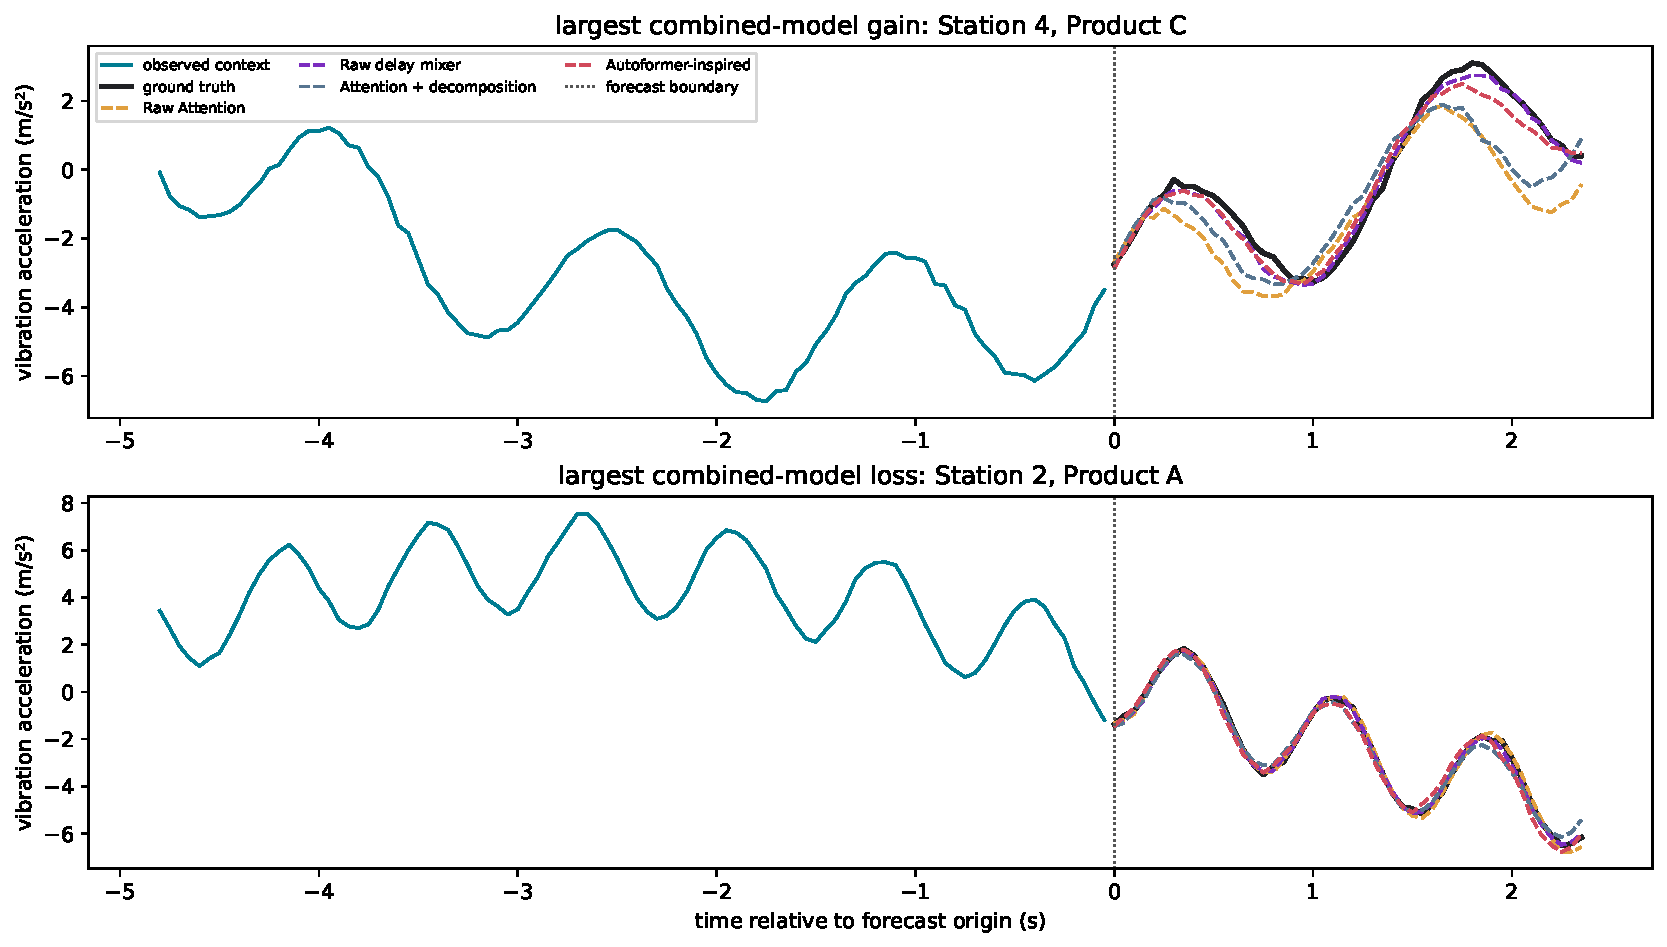
\includegraphics[width=0.75\linewidth]{figures/task1/4.1-1.pdf}
\caption{Output 4.1: validation windows with the largest gain (station 4, Product C) and largest loss (station 2, Product A) of the Autoformer-inspired model over Raw Attention.}
\end{figure}

\begin{figure}[H]\centering
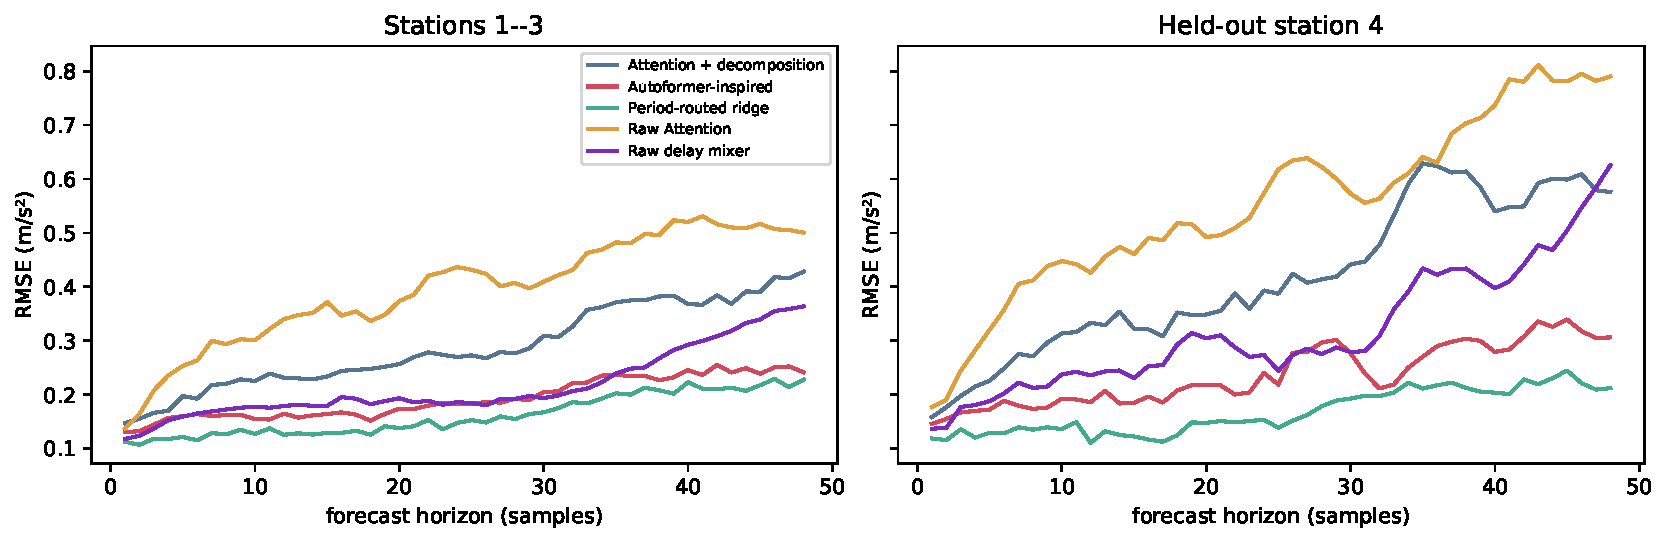
\includegraphics[width=0.85\linewidth]{figures/task1/4.2-1.pdf}
\caption{Output 4.2: validation RMSE along the 48-step horizon, established stations (left) and station 4 (right).}
\end{figure}

\textbf{(a) Prediction} (recorded before Output 4.1). Decomposition should help most on contexts where the slow component is prominent, because it removes the ramp before the mixer sees it. Delay mixing on a raw, ramp-dominated context would score delays by ramp-dominated correlations.

\textbf{(b) Evidence} (validation). On established stations, each switch helps in both settings; delay mixing is the larger in both. The gains overlap: together they gain less than their sum (interaction $-0.081$ in RMSE, $-0.065$ in MSE), and station~4 agrees. On high-drift contexts, delay mixing still gains far more than decomposition, so my prediction is not supported. Along the horizon, errors start at 0.11--0.15. By step 48, Raw Attention reaches 0.50, while routed ridge (0.23) and the Autoformer-inspired model (0.24) stay lowest in both populations.

\textbf{(c) Deployment.} I chose period-routed ridge for both populations, from validation, before Output 4.3. It has the lowest validation MSE and RMSE on established stations (0.028 / 0.166) and on station~4 (0.030 / 0.173). It uses 16\% of the neural models' parameters, fits in closed form in milliseconds, and needs no station identity. Its risk is reliance on hand-set pace bands. Its test RMSE (0.161 established, 0.183 station~4) confirms the choice.

\begin{table}[H]\centering\small
\caption{Output 4.3: the selected models on validation and test.}
\begin{tabular}{llrrrr}
\toprule
Population & Model & Val.\ MSE & Val.\ RMSE & Test MSE & Test RMSE \\
\midrule
Established & Period-routed ridge & 0.0275 & 0.166 & 0.0260 & 0.161\\
Held-out station 4 & Period-routed ridge & 0.0298 & 0.173 & 0.0333 & 0.183\\
\bottomrule
\end{tabular}
\end{table}

\paragraph{Task 1 in one sentence.} On this benchmark the right inductive bias beat flexibility: a linear map conditioned on the pace outperformed every learned design on both populations (validation), and the best neural model, the Autoformer-inspired one, approaches it only by learning a soft version of the same idea, organizing the window by its period.
